\chapter{Apéndices}

\newpage
\section{Documentación del \textit{hardware}}
\subsection{Generación de LUTs para NTCs}
\begin{lstlisting}[language=Matlab, basicstyle=\ttfamily\small, breaklines=true, frame=single]
%% Temperature sensing LUT calculation for DFS05HF12EYR1
clc, clear
%% Initial variables
temperatures = 0:10:120; % Temperature array, 0.01degC resolution [degC]

%% NTC Parameters

% DFS05HF12EYR1 internal NTC
% Beta is a function of temperature

%beta_values = [3375, 3411, 3433]; % Beta values for different temperatures [K]
%beta_temps = [50, 80, 100]; % Temperatures for the different beta values [degC]

% CAB016M12FM3 internal NTC
% Beta is a function of temperature
beta_values = [3380, 3468, 3523]; % Beta values for different temperatures [K]
beta_temps = [50, 80, 100]; % Temperatures for the different beta values [degC]

% Both very similar, interchangable

beta_coeffs = polyfit(beta_temps, beta_values, 1); % Fit the beta deviation with linear regression

beta_temp = polyval(beta_coeffs,log(temperatures+1e-9)); % Beta is evaluated for all temperatures, avoiding 0degC [K]

T_0 = 25; % T at which NTC = R0 [degC]

R_0 = 5e3; % NTC resistance value at T_0 [R]

%% Calculations

% NTC resistance value for all temperatures, with varying beta
NTC = R_0*exp(-beta_temp.*(1./(273.15+25)-1./(273.15+temperatures))); % NTC resistance with no errors [R]

% Reading using UCC21732 isolated analog reading. 200uA current source 
R_filt = 10e3; % Filter resistance, in series with the NTC [R]

I_AIN = 200e-6; % Internal current source [A]
V_AIN = I_AIN * (R_filt + NTC); % Sensed voltage [V]

D = -20 * V_AIN + 100; % Duty cycle out [%]

VCC_GD = 5; % GD supply voltage [V]
V_read = VCC_GD * D/100; % Voltage read by ADC [V] (filtered with ideal RC)

VCC_ADC = 3.3; % MCU/ADC supply voltage [V]
bits = 12; % ADC bits [b]

bits_read = ceil(V_read * (2^bits) / VCC_ADC); % MCU/ADC read bits [b]
bits_read(bits_read>2^bits)=2^bits; % Saturation to 2^bits
bits_read(bits_read<0)=0; % Saturation to 0

% Create the plot
figure;
plot(temperatures, bits_read, 'LineWidth', 4);

% Add labels and title
xlabel('Temperature (degC)', 'FontSize', 12);
ylabel('Bits Read', 'FontSize', 12);
title('Bits Read vs. Temperature', 'FontSize', 14);

% Add grid and adjust limits
grid on;
xlim([min(temperatures)-5, max(temperatures)+5]);
ylim([min(bits_read)-50, max(bits_read)+50]);

% Customize the appearance
set(gca, 'FontSize', 10); % Adjust font size for axis labels
set(gca, 'LineWidth', 1.5); % Adjust axis line width

OUTPUT_LUT = [temperatures; bits_read];

\end{lstlisting}

\subsection{Dimensionado de las resistencias de descarga}

\begin{lstlisting}[language=Python, basicstyle=\ttfamily\small, breaklines=true, frame=single]
import itertools
import math

# Given data
target_resistance = 20000  # 18kR
tolerance = 1000  # +-1kR
power_rating = 20  # 20W
voltage = 600  # 600V
capacitance = 100e-6  # 100uF
Vf = 60  # 60V

# E-12 resistor values in R
e12_values = [1.0, 1.2, 1.5, 1.8, 2.2, 2.7, 3.3, 3.9, 4.7, 5.6, 6.8, 8.2]
multipliers = [10 ** x for x in range(6)]

# SMD packages with their corresponding wattage
smd_packages = {
	"1206": 0.25,
	"1210": 0.5,
	"2010": 0.75,
	"2512": 1
}


# combination = [value, number of parallel resistors]

def calculate_resistance(combination):
return combination[0] / combination[1]


def calculate_power_dissipation(combination):
power_dissipation = voltage ** 2 / combination[0]
return power_dissipation


def calculate_discharge_time(combination):
resistance = calculate_resistance(combination)
discharge_time = resistance * capacitance * math.log(voltage / Vf)
return discharge_time


def find_parallel_combinations(target_resistance, tolerance, power_rating):
all_combinations = []
for r_value in e12_values:
for multiplier in multipliers:
base_resistance = r_value * multiplier
for num_parallel in range(1, 101):  # Assuming a maximum of 100 parallel resistors
current_resistance = base_resistance / num_parallel
if target_resistance - tolerance <= current_resistance <= target_resistance + tolerance:
for package, wattage in smd_packages.items():
power_dissipation = calculate_power_dissipation([base_resistance, num_parallel])
if power_dissipation <= wattage:
discharge_time = calculate_discharge_time([base_resistance, num_parallel])
power_percentage = (power_dissipation / wattage) * 100
all_combinations.append((base_resistance, num_parallel, package, power_dissipation, discharge_time, power_percentage))
return all_combinations


if __name__ == "__main__":
combinations = find_parallel_combinations(target_resistance, tolerance, power_rating)
print("Possible combinations:")
for combo in combinations:
print(f"Resistance: {round(combo[0]/1000)}kR, n: {combo[1]}, SMD Package: {combo[2]}, "
f"P_diss: {round(combo[3], 3)} W, t_dis: {round(combo[4], 3)} s, "
f"Power: {round(combo[5], 2)}% of package maximum")
	
\end{lstlisting}

\subsection{Cálculo de divisores de tensión estandarizados}

\begin{lstlisting}[language=Python, basicstyle=\ttfamily\small, breaklines=true, frame=single]
import itertools

# Define resistor series and their respective multipliers
resistor_series = {
	'E6': [1.0, 1.5, 2.2, 3.3, 4.7, 6.8],
	'E12': [1.0, 1.2, 1.5, 1.8, 2.2, 2.7, 3.3, 3.9, 4.7, 5.6, 6.8, 8.2],
	'E24': [1.0, 1.1, 1.2, 1.3, 1.5, 1.6, 1.8, 2.0, 2.2, 2.4, 2.7, 3.0, 3.3, 3.6, 3.9, 4.3, 4.7, 5.1, 5.6, 6.2, 6.8, 7.5, 8.2, 9.1],
	'E48': [1.00, 1.05, 1.10, 1.15, 1.21, 1.27, 1.33, 1.40, 1.47, 1.54, 1.62, 1.69, 1.78, 1.87, 1.96, 2.05, 2.15, 2.26, 2.37, 2.49, 2.61, 2.74, 2.87, 3.01, 3.16, 3.32, 3.48, 3.65, 3.83, 4.02, 4.22, 4.42, 4.64, 4.87, 5.11, 5.36, 5.62, 5.90, 6.19, 6.49, 6.81, 7.15, 7.50, 7.87, 8.25, 8.66, 9.09],
}

# Define tolerance values
sum_tolerance = 10000  # 10k ohms
# Target values
target_sum = 100000  # 100k ohms

Vout = 4
Vout_error = 0.15

# Function to generate resistor values for a given series
def generate_resistor_values(series):
return resistor_series[series]
# Function to calculate the closest combination
def find_closest_combination(Vout, Vout_error):
closest_sum = None
closest_combination = None
lowest_series_combination = None
comb_number = 0
for series, values in resistor_series.items():
for multiplier in values:
resistor_values = generate_resistor_values(series)
for combo in itertools.combinations(resistor_values, 2):
R1, R2 = combo
comb_number += 1

sum_resistors = (R1 + R2) * 10000  # in ohms
if Vout >  1.186 * 2:
actual_Vout = 1.186 * (1 + R2 / R1)
else:
actual_Vout = 1.186 * (1 + R1 / R2)
Vout_diff = Vout - actual_Vout

# Check if the sum is within +/- 10kR and the Vout error is within the specified tolerance
if ((target_sum - sum_tolerance) <= sum_resistors <= (target_sum + sum_tolerance)) and (Vout_diff <= Vout_error and Vout_diff > 0):
if closest_sum is None or abs(sum_resistors - target_sum) < abs(closest_sum - target_sum):
closest_sum = sum_resistors
if Vout >  1.186 * 2:
closest_combination = (series, R1, R2, actual_Vout)
else:
closest_combination = (series, R2, R1, actual_Vout)

if lowest_series_combination is None or series < lowest_series_combination[0]:
if Vout >  1.186 * 2:
lowest_series_combination = (series, R1, R2, actual_Vout)
else:
lowest_series_combination = (series, R2, R1, actual_Vout)

return closest_combination, lowest_series_combination, comb_number



# Find the closest combination
closest_combination, lowest_series_combination, comb_number = find_closest_combination(Vout, Vout_error)

# Print the result
if closest_combination:
series, R1, R2, actual_Vout = closest_combination
print("Closest combination found:")
print("Series:", series)
print("R1 =", R1*10, "kOhms")
print("R2 =", R2*10, "kOhms")
print("Vout =", actual_Vout, "V")
else:
print("No combination found within the specified Vout error.")

if lowest_series_combination:
series, R1, R2, actual_Vout = lowest_series_combination
print("Lowest series combination found:")
print("Series:", series)
print("R1 =", R1*10, "kOhms")
print("R2 =", R2*10, "kOhms")
print("Vout =", actual_Vout, "V")
else:
print("No combination found using the lowest series.")

print("A total of ", comb_number, " combinations were checked")
\end{lstlisting}
\subsection{Documentación de \textit{Inverter\_Power} (Leapers)}
\includepdf[pages=-, landscape=true]{../HW/Inverter_Power/Project Outputs for Inverter_Power/Inverter_Power-Leapers.PDF}
\subsection{Documentación de \textit{Inverter\_Power} (Wolfspeed)}
\includepdf[pages=-, landscape=true]{../HW/Inverter_Power/Project Outputs for Inverter_Power/Inverter_Power-Wolfspeed.PDF}
\subsection{Documentación de \textit{Inverter\_Control}}
\includepdf[pages=-,landscape=true]{../HW/Inverter_Control/Project Outputs for Inverter_Control/Inverter_Control.PDF}

\newpage
\section{Documentación del \textit{firmware}}
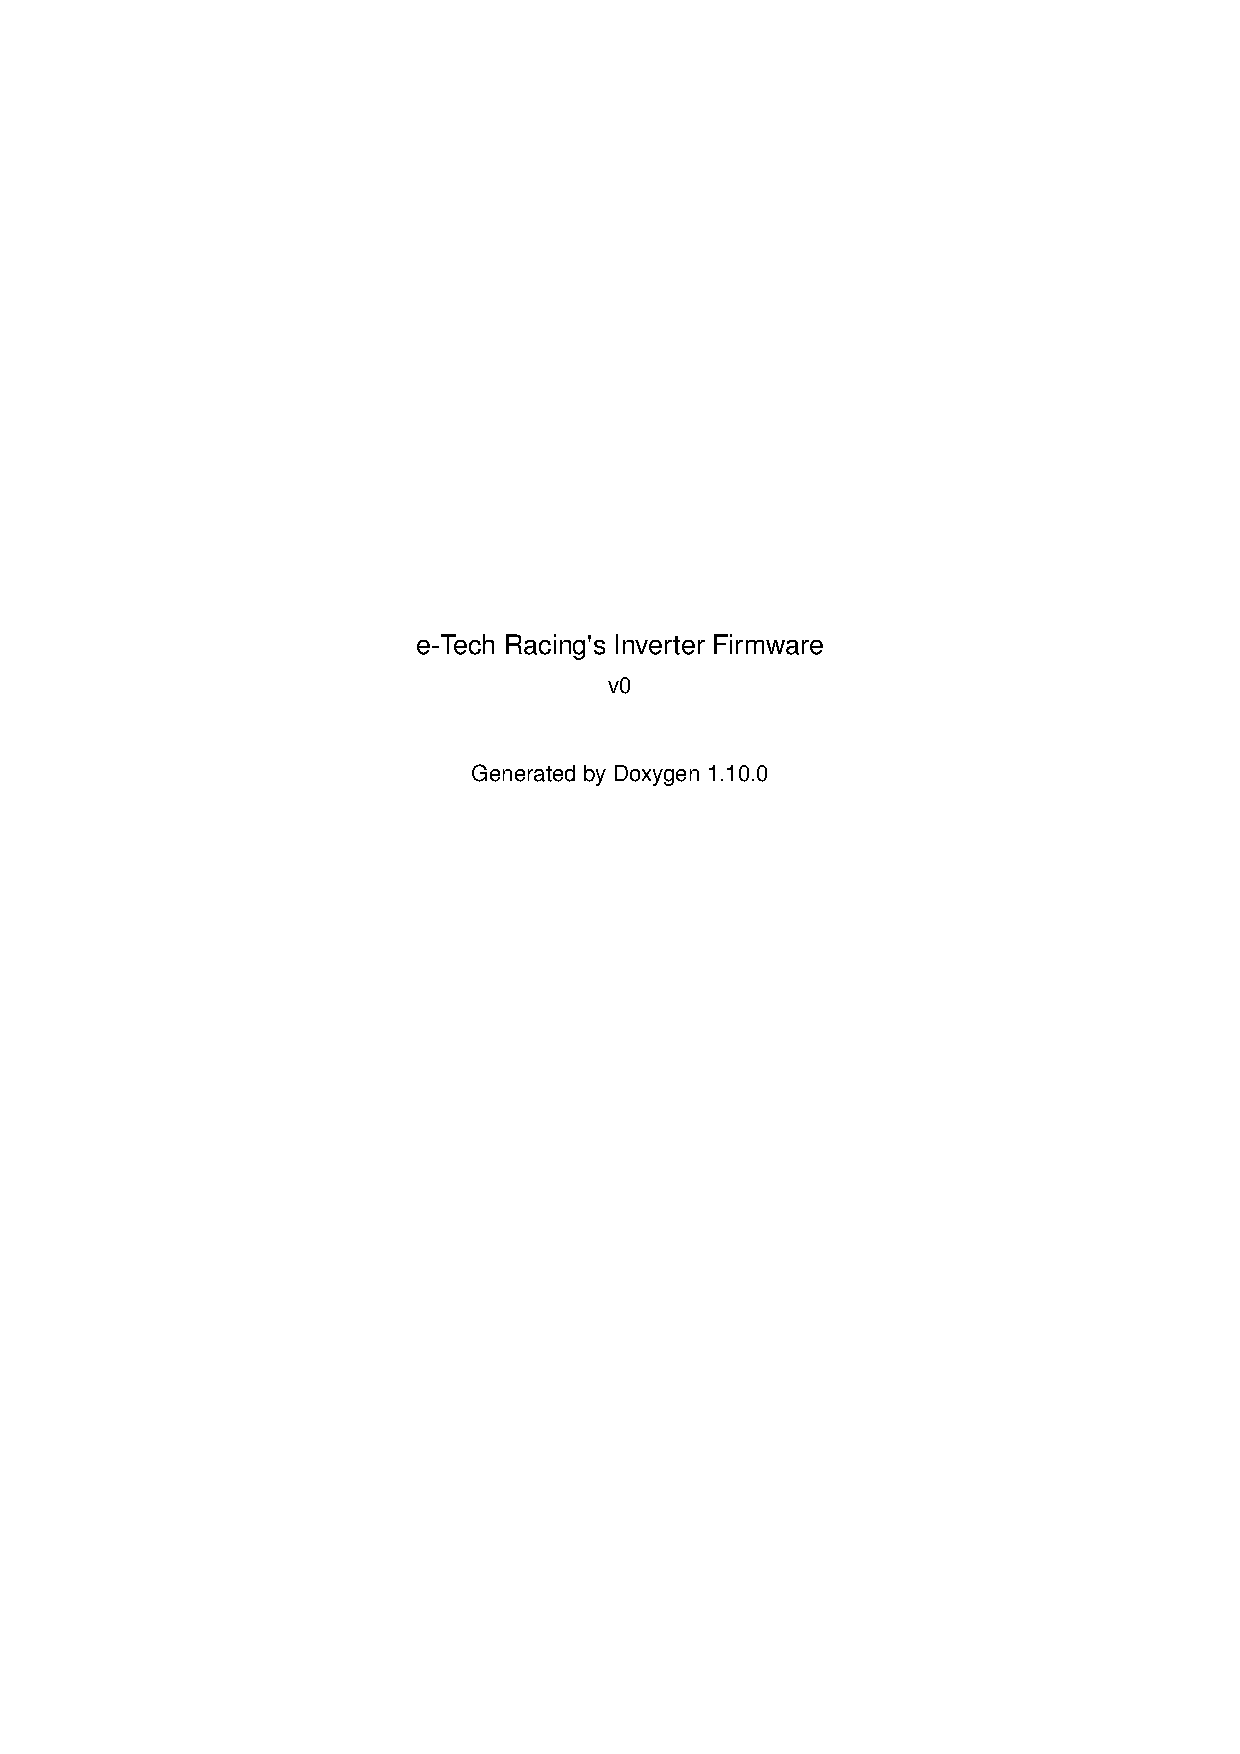
\includepdf[pages=-]{../SW/Documentation/latex/refman.pdf}
